\documentclass[12pt,oneside,a4paper]{report}
\usepackage{mathtools}
\usepackage[HTML, hyperref, svgnames, table]{xcolor}
\usepackage[utf8]{inputenc}
\usepackage{polski}
\usepackage[polish]{babel}
\usepackage{multicol}
\usepackage{graphicx} 
\usepackage[margin=1in]{geometry}
\usepackage[linesnumbered,ruled,vlined]{algorithm2e}
\usepackage{booktabs}
\usepackage{tabularx}

\begin{document}
\begin{titlepage}
   \begin{center}
        \vspace*{2cm}

        \large Politechnika Wrocławska Wydział Elektroniki Kierunek Teleinformatyki
        \vspace*{2cm}

        \large Inżynierska praca dyplomowa

        \vspace*{0.5cm}
        \huge\textbf{Projekt sztucznej inteligencji}

        \vspace{0.5cm}
        \normalsize 
            
        \textbf{Michał Żarejko}
        \vspace{3cm}

   \end{center}

        \setlength{\columnsep}{-20pt}
        \begin{multicols}{2}
           Dyplomant:  

           \vspace{0.2cm}
           Nr albumu:

           \vspace{0.2cm}
           Promotor:

        \columnbreak
           \textbf{Michał Żarejko}

           \vspace{0.2cm}
            \textbf{249374}

           \vspace{0.2cm}
            \textbf{dr inż. Paweł Zyblewski}
        \end{multicols}

        \vspace{0.5cm}


        \vspace{2cm}
   \begin{center}
        Wrocław. 2021


   \end{center}
\end{titlepage}


\newgeometry{top=2.5cm,bottom=2.5cm,right=2.5cm,left=2.5cm}
\tableofcontents{}
\newpage

\setlength{\parindent}{0.5em}
\setlength{\parskip}{0.5em}
\renewcommand{\baselinestretch}{2.0}

\chapter{Wstęp}

Duży rozwój nauki w ostatnich latach związany z uczeniem maszynowym, spowodował powstanie wielu
nowoczesnych algorytmów i technologi, które pomagają aktualnie w codziennych czynnościach lub 
zastępują ludzi w odpowiedzialnych procesach. 

Można wymienić dzisiaj wiele rozwijanych narzędzi związanych z uczeniem maszynowym, które
są używanych w życiu
prywatnym. Są to między innymi asystenci głosowi, tłumacze językowe, modele wyświetlające elementy na
stronach internetowych na podstawie gustu użytkownika, gry wideo lub inteligentne samochody.
Dodatkowo sztuczna inteligencja jest mocno wykorzystywana w wielu firmach, między 
innymi na halach produkcyjnych, w transporcie, medycynie, cyberbezpieczeństwie. 
Po mimo tylu możliwości i zastosowań, omawiany temat zyskuje największą popularność
medialną przez gry rywalizacyjne, gdzie głównym zadaniem jest pokazanie przewagi algorytmów względem
ludzi. W ostatnich latach doszło do wielu wydarzeń gdzie profesjonalni gracze 
musieli stoczyć pojedynek z wytrenowaną sztuczną inteligencją. 


Między innymi w 2016 roku zorganizowano
mecz między Fan Hui, mistrzem Europy w chińskiej grze Go oraz algorytmem AlphaGo \cite{Go}.
Model utworzony przez zespół DeepMind osiągnął duży sukces przez wygraną z przeciwnikiem.
Do tej pory gra była uważana powszechnie za skomplikowaną i trudną do rozwiązania.

W 2019 roku utworzono model zwany OpenAI Five czyli pierwsze na świecie AI, które pokonało
mistrza świata Team OG w rywalizacji typu e-sport \cite{Dota2}. Gra Dota 2 polega na rywalizacji 5-osobowych
zespołów na okreslonej mapie.
Wydarzenie było mocno omawiane w mediach z powodu pierwszego takiego osiągnięcia w skali światowej
oraz skąplikowania gry. 
Dla porównania środowisko Go zawiera 150 możliwych ruchów na turę, Dota 2
może posiadać ich 20 000 w czasie 45 minut \cite{Dota2}.


Takie wydarzenia pokazały, że w dzisejszych czasach sztuczna inteligencja może przewyrzszać
myśleniem strategicznym człowieka.
Często w tworzeniu takich programów dużym wyzwaniem jest poziom skomplikowania gry. 
Zależy to między innymi od typu środowiska, deterministycznego lub stochastyczne, 
od poziomu dynamiki gry lub od tego czy przestrzeń wymiarowa jest
dyskretna lub nieskończona.
Aktualnie jednak jednym z największych problemów takich programów jest niedostateczny
zakres dostępnych informacji o środowisku. Sztuczna inteligencja, aby zwyciężać
musi zostać nauczona grać, więc potrzebuje dużej ilości danych wejściowych, które są 
rozróżnialne. Przykładem gry, która jest pozbawiona tego problemu są szachy. 
Sztuczna inteligencja wykonuje ruchy bazując na informacjach w jaki sposób są ułożone pionki
w danym momencie i na historii dotychczasowej gry. Zmiana stanu środowiska jest
zauważalna przez gracza co pozwala na natychmiastową reakcję i prostsze sposoby na uczenie
maszynowe. Przykładem gry ciężkiej do rozwiązania, w której występuje nie pełny zestaw informacji 
jest Poker Texas Holdem, po mimo wiedzy o kartach w ręce i na stole, gracz nie posiada wiedzy o 
kartach przeciwników, w takim przypadku dwa pozornie identyczne stany środowiska w
rzeczywistości mogą się różnić. Z powodu takich cech większość popularnych algorytmów jak 
DQN, Actor-Critic lub AlphaZero staje sie bezużyteczna i nie daje dobrych rezultatów.

W niniejszej pracy przedstawiono sposób możliwego rozwiązania takiego problemu przy pomocy 
algorytmu o nazwie Deep CFR. Pierwszy i drugi rozdział dokładnie opisuje cele pracy, zakres 
projektu, 
oraz zagadnienia wymagane aby zrozumieć działanie algorytmu. W trzecim rozdziale skupiono się na
implementacji, czwarty pokazuje uzyskane wyniki.


\section{Cel i zakres pracy}

Głównym celem pracy jest implementacji algorytmu Deep CFR do gry Heads Up Limit Texas 
Poker Hold'em. Jest to popólarna wersja rozgrywki 2-osobowej gdzie uczestnicy nie mogą wybrać
samodzielnie kwoty podbicia stawki, jest ona ograniczona przez ustaloną wartość. Takie środowisko
minimalizuje możliwe ruchy do 3 akcji. Używając omawianego algorytmu
wytrenowano 5 modeli rozpoznawania, które zostały następnie wykorzystane do rozegrania
turnieju składającego się na wszystkie kombinacje rozgrywek modeli po
10 powtórzen gry. Taki proces pozwoli określić, który model wydaje się najbardziej dopracowany. 

\section{Teoria oraz istniejące rozwiązania gry}

W ciągu ostatnich 10 lat powstało wiele algorytmów rozwiązujących różne werjse gry Poker.
Miedzy innymi Counterfactual Regret Minimization,Extensive-Form Fictitious Play, 
Neural Fictitious Self-Play wykorzystujący sieci neuronowe  oraz algorytm DQN lub
Regret Policy Gradients. Pierwszy z wymienionych, CFR powstał w 2007 roku i był jednym z pierwszych 
pomyślną próbą rozwiązania środowiska Texas Hold'em \cite{rmg}. To na jego podstawie utworzono wiele nowoczesnych
algorytmów, które dają szanse rozwiązać takie środowiska jak HULH \cite{eq}. W 2010 roku powstał algorytm XFP testowany na 
prostszej wersji gry Texas Hold'em \cite{FSEG}. Innym istniejącym algorytmów jest
Regret Policy Gradients oparty na MDP.
Z wymienionych algorytmów zaimplementowanym rozwiązaniem w niniejszej pracy jest CFR 
rozszerzony o sieci neuronowe,
zwany Deep CFR z wersją gry Heads Up Limit Texas Hold'em. Daje on szybką zbierzność,
dodatkowo jest prostszy i wymaga mniejszej mocy obliczeniowej niż bazowy 
CFR \cite{dcfr}.

\subsection{Analiza Texas hold'em Poker}

Omawiana gra jest jedną z najpopularniejszych rywalizacji występujących w kasynach, dodatkowo jest to
dominująca gra hazardowa. Można ją zcharakteryzować tym, że jest nie deterministyczna oraz częściowo 
obserwowalna \cite{sp}.  


Przez takie cechy gra była od zawsze tematem sporów, czy na jej wynik ma większy wpływ
losowość czy umiejętności. Jak wynika z badań dużym aspektem pomagającym w osiągnięciu zwycięstwa 
jest panowanie na emocjami, dokładna analiza stanu gry oraz umiejętność opuźnienia natychmiastowej
nagrody z możliwością jej zwiększenia w puźniejszych turach oraz pamięć o wynikach z poprzednich 
rund \cite{gm}. 

\begin{figure}[h!]
            \center
           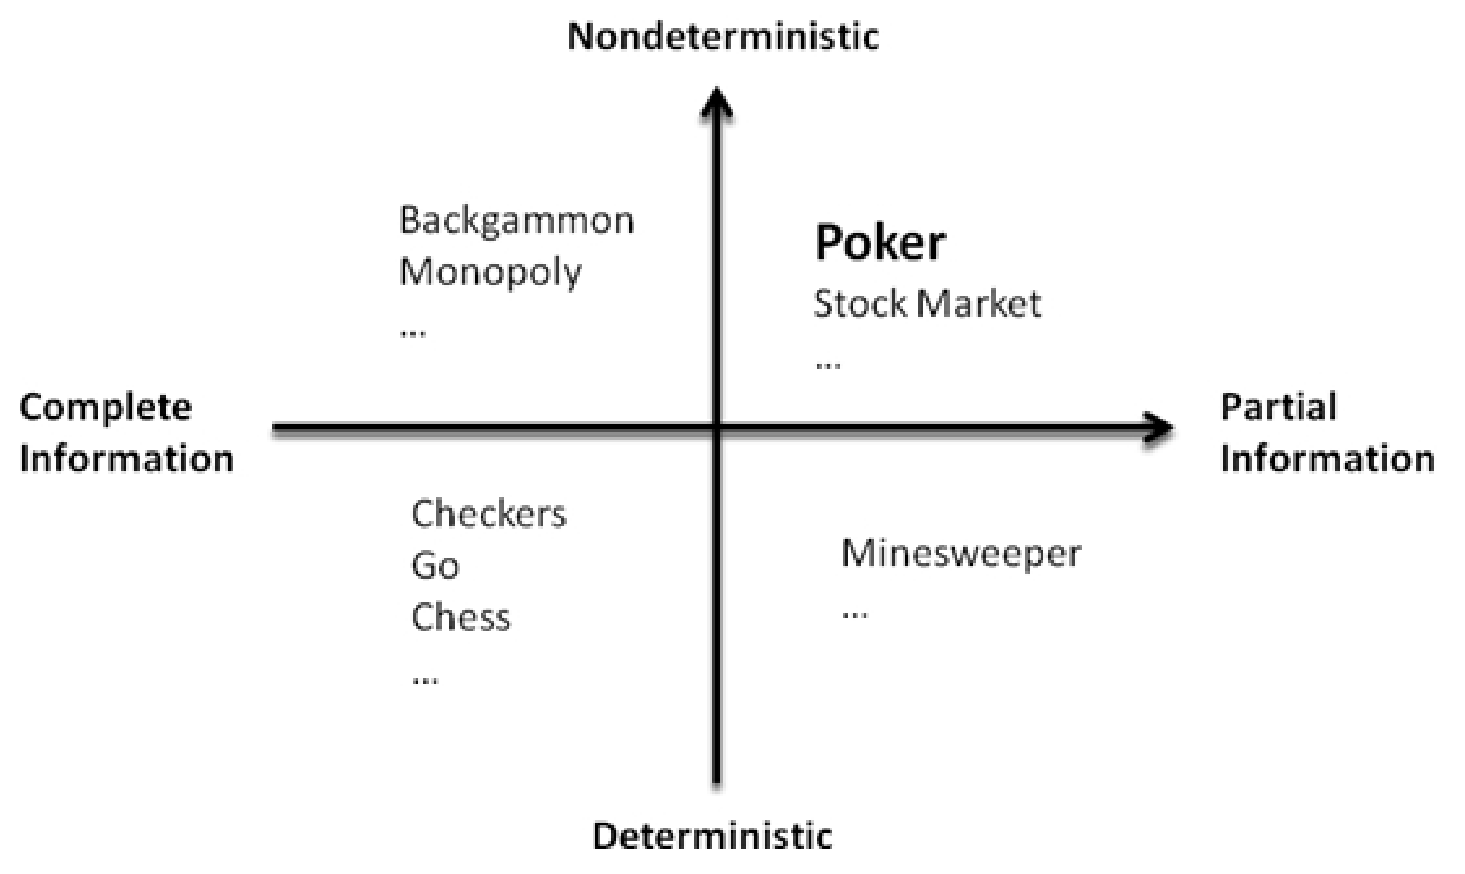
\includegraphics[width=0.5\textwidth]{./img/classification.pdf}
           \caption{Podział typów gier \cite{sp}.}
\end{figure}

Dodatkowo ważnym elementem jest wybrana strategia przez uczestnika. Na podstawie
wybieranych akcji, można sklasyfikować gracza na cztery kategorie. 

\subsubsection{Loose Passive}

Osoba, która bardzo często wchodzi do gry nie zależnie czy karty, które posiada dają jej
niskie szanse na wygraną. Ten typ gry charakteryzuje się częstym wykonywanie akcji 'call' oraz
małą ilością przebić stawki niezależnie od posiadanych kart. 
Najlepszym sposobem przeciw taki graczom jest przebijanie stawki tylko
kiedy ma się dobre karty, a w innym przypadku nie należy wchodzić do gry \cite{class}.

\subsubsection{Loose Aggressive}

Ten typ gry okresla osobę, która często wykonuje akcję 'raise' i 're-raise' 
pod warunkiem, że ma silne karty, w innym przypadku wyrównuje żetony do aktualnej stawki.
Taka strategia okazuje się nie efektywna w przypadku gry z osobami, które często wchodzą do gry nie 
zależnie od kart jak na przykład typ 'Loose-Passive'. Aby wygrać z taką osobą najlepiej 
przebijać stawke aż do rundy 'river' \cite{class}.

\subsubsection{Tight Passive}

Można poznać tą kategorię gry przez to, że uczestnik wchodzi tylko z dobrymi kartami i często 
pasuje przy spotkaniu z graczem agresywnym, który przebija. Taki gracz traci wiele okazji, kiedy
mogł by wygrać. Dobrą strategią przeciw nim jest granie pasywnie w przypadku kiedy przebijają stawkę
w turze 'turn' lub 'river', w innym przypadku gra agresywnie jest dobrą opcją \cite{class}.


\subsubsection{Tight Aggressive}

Typ gry popularny wśród profesjonalnych graczy, grają jak typ 'Tight Passive' w rundzie 'flop',
potem zmieniają ten styl na inny \cite{class}.
Dobymi rozwiązaniami przeciw takim graczom jest pruba 'blefowania', kiedy oponent zaczyna grać
agresywnie \cite{class}.




\begin{figure}[h!]
            \center
           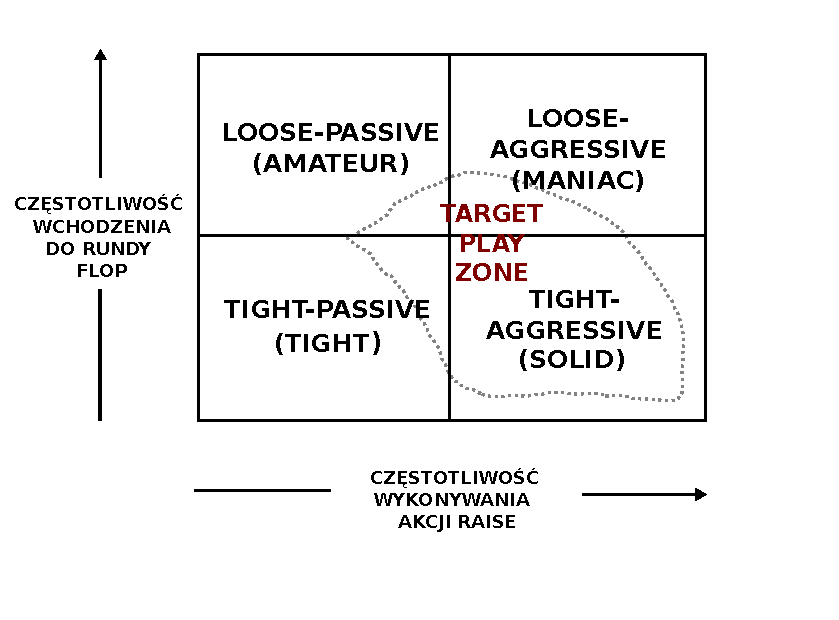
\includegraphics[width=0.5\textwidth]{./img/class.pdf}
           \caption{Podział graczy \cite{class}.}
\end{figure}


Jak wynika z powyrzszych faktów, gra 'Poker Texas Hold'em' zawiera wiele elementów nie związanych z
losowością, gdzie dobieranie odpowiedniej strategi do typu gracza pełni kluczową rolę. W takim
wypadku jest uzasadnione wysunięcie tezy, że można utworzyć sztuczną inteligencję mogącą wygrywać w
pokera z ludzmi.

\subsection{Uczenie przez wzmacnianie}

Jest wiele sposobów na tworzenie sztucznej inteligencji do gier, między innymi mozna użyć technik uczenia
nadzorowanego pod warunkiem jeśli przygotuje się odpowiednie zbiory danych. W pracy jednak
zdecydowano się na uczenie przez wzmacnianie. Wynika to z faktu, że jest mało publicznych zapisów
gry profesjonalnych graczy, które mogły by posłużyć jako zbiory uczące. Algorytmy należące do
wybranego działu uczenia maszynowego powinny być w stanie uczyć się na podstawie interakcji ze
środowiskiem.  


\subsection{Teoria Gier}

Aby zrozumieć działanie wymienionych algorytmów nalerzy zapoznać się
działem matematyki o nazwie "Teoria Gier" . Bada on optymalne zachowanie w grach
hazardowych przez dobieranie odpowiedniej strategii bazującej na zasadzie "Równości Nasha" oraz 
opisie środowiska jako gry w postaci ektensywnej \cite{gt}.

\subsubsection{Gra w postaci ekstensywnej}

Gry w
formie ekstensywnej można przedstawić jako drzewo decyzyjne gdzie każdy węzeł rozgałęzia się na
możliwe akcje oraz identyfikuje aktualny stan gracza przez zestaw informacji I,
ostatnie węzły to stany końcowe gdzie określony gracz zyskuje nagrode lub ją traci. Jest to sposób
na uproszczony opisu gry.

\begin{figure}[h!]
  \centering
  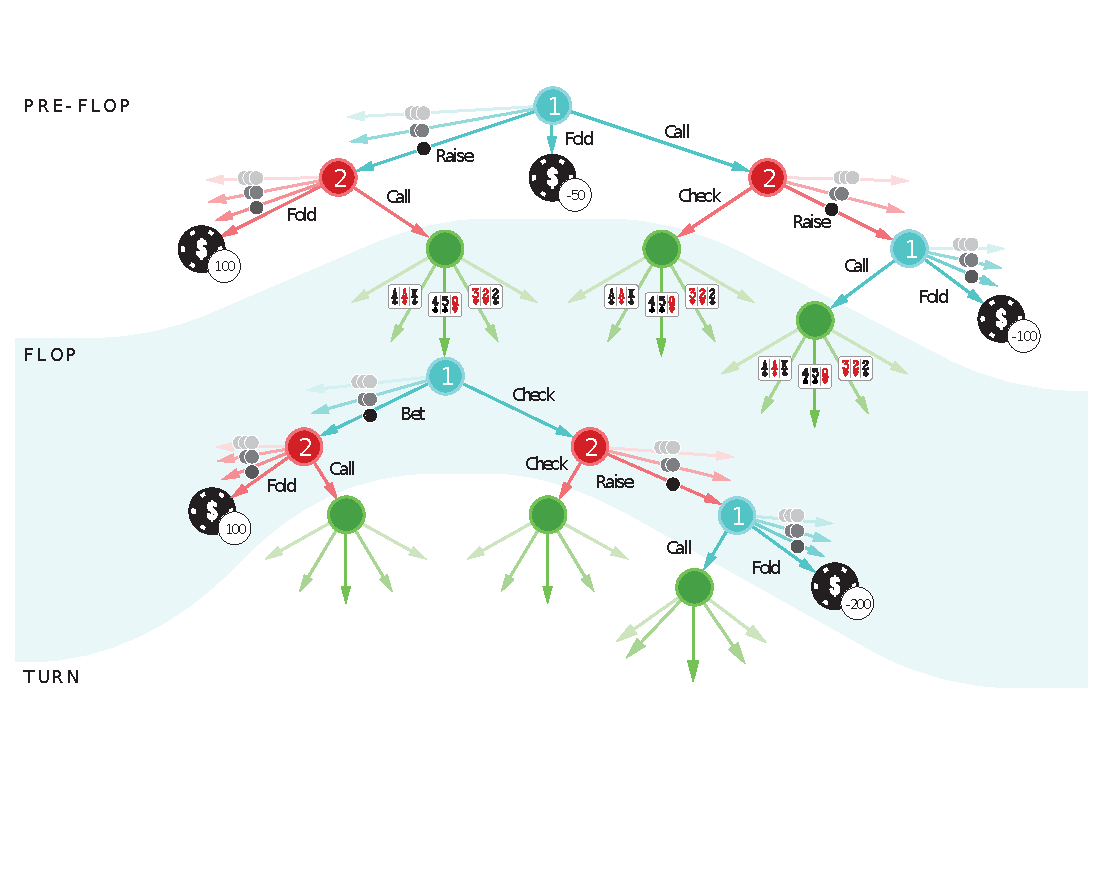
\includegraphics[width=0.7\textwidth]{./img/tree1.pdf}
  \caption{Drzewo decyzyjne gry "No-limit Poker Texas Hold'em". \cite{ds}}
\end{figure}


\subsubsection{Równość Nasha}

W grach to twierdzenie określa perfekcyjny stan gry gdzie wszyscy gracze wykorzystują najlepszy
zestaw strategii, którego zmiana przyniesie tylko straty. Oznacza to, że nie jest możliwe
zwiększenie uzyskanej nagrody bedąc w tym stanie \cite{gt}.

\subsubsection{Zero-sum}

W pracy założono, że "Heads Up Poker Texas Hold'em" jest grą
2-osobową o sumie zerowej, czyli wygrana jednego
uczestnika oznacza całkowitą porażkę oponenta w wyskokości wygranej stawki w taki sposób, że suma 
wygranej i przegranej wynosi zero.
W takiej formie można
zaimplementować Deep CFR, który ma szanse zbiec się do stanu bliskiego "Równości Nasha" \cite{dcfr}.
Algorytm będzie przez wiele iteracji eksplorował drzewo decyzyjne i dobierał odpowiednie 
strategie aż trafi na takie, które dają najlepsze rezultaty.


\subsection{Historia modeli Texas Hold'em Poker}

Bazując na teorii gier oraz różnych algorytmach powstało wiele rozwiązań różnych wersji gry Poker.
Pierwsze dokumenty naukowe omawiały bardzo proste
środowiska jak Poker Kuhn.
Dopiero w 2015 roku utworzono pierwszą znaną sztuczną inteligencję Cepheus rozwiązującą problem
Heads Up Limit Texas Hold'em wykorzystujące algorytm CFR+. Po tym osiągnięciu rozpoczęto prace nad
algorytmem mogącym rozwiązać problem gry Heads Up No-limit Texas Hold'em. Zajeło to 2 lata od 
Cepheus'a, model nazwano "DeepStack", mieszał on techniki znane z Deep CFR. 
Przetestowano go na 33 profesjonalnych graczach w wielu iteracjach gry. Algorytm w większości
przypadków wygrał \cite{ds}. Była to pierwsza wygrana AI z człowiekiem w najtrudniejszej wersji gry Poker.

\section{Counterfactual Regret Minimization}

\subsection{Regret Matching}

Jest to metoda uczenia polegająca na minimalizacji żalu używana w algorytmie CFR.
Opisuje się to jako sposób na liczenie wektorów wag o długości równej liczbie możliwych akcji A
, korztstając z $u^{t}$ czyli nagrody uzyskanej w stani t oraz z dystrybucji ruchów $p^{t}$ \cite{rmg}. 
Posiadając te informacje algorytm iteracyjnie aktualizuje wagi wzorem 2.1.


\begin{equation}
p^{t}_{i}\left( a \right) = \left\{ \begin{array}{ll}
      \frac{R^{t-1, \text{+}}\left(a\right)}{ \Sigma_{a' \in A} R^{t-1,\text{+}}\left(a'\right)} &
      \mbox{if $\Sigma_{a' \in A} R^{t-1,\text{+}}\left(a'\right) >
      0$};\\
      \frac{1}{|A|} & \mbox{$otherwise$}.\end{array} \right. \ 
\end{equation}

Gdzie $R^{t} \text{(a)}$ jest równe formule 2.2, a $R^{t,\text{+}}(a)$ oblicza się jak w 2.3.

\begin{equation}
   R^{t} (a) = \frac{1}{T} {\sum_{t=1}^{T} u^{t} (a)} - \sum_{a \in A} p^{t} (a) u^{t} (a)
\end{equation}

\vspace{1cm}
\begin{equation}
   R^{t,\text{+}}(a) = max(R^t(a),0)
\end{equation}

Podsómowując pwyżesze wzory, dla każdej akcji wektora w danym stanie wylicza się $R^{t}(a)$, gdzie
należy skorzystać z sumy przyszłych wartości $u^{t}(a)$ oraz $p^{t}(a)$ 
dla wybrania danych ruchów. Całość obrazuje jak bardzo gracz żałuje wybranych
akcji w czasie od t.

\subsection{Regret Minimization}

W przypadku algorytmu CFR i gry Heads Up Limit Texas Hold'em gracz ma do zynienia z wyborem strategi
$\sigma_{i}^{t}$ dlatego wylicza się wartość zwaną 'Average overall regret', która określa jak gracz
i będzie żałował wybór danej strategi aż do czasu T \cite{rmg}.

\begin{equation}
   R^{T}_{i} = \frac{1}{T} \max_{\sigma^{*}_{i} \in \Sigma_{i}} \sum_{t=1}^{T}
   \left(u_{i}\left(\sigma_{i}^{*}, \sigma_{-i}^{t}\right) - u_{i}(\sigma^{t})\right)
\end{equation}

Głównym zadaniem algorytmu CFR jest minimalizacja tej wartości dla wszystkich graczy.
Dodatkowo dla każdego gracza oblicza się średnią strategię dla 
każdego stanu I oraz akcji A czyli sumę wszystkich strategi, które posiada gracz aż do stanu T
podzielone przez sumę prawdopodobieństw $\pi^{\sigma^{t}}_{i}$ osiągnięcia stanów I dla
strategi $\sigma^{t}$ \cite{rmg}.

\begin{equation}
   \sigma^{-t}_{i} \left(I\right) \left(a\right) = \frac{\sum^{T}_{t=1} \pi^{\sigma^{t}}_{i}
   (I)\sigma^{t}(I)(a)}{\sum^{T}_{t=1} \pi^{\sigma^{t}}_{i}(I)}
\end{equation}

Jesli wszyscy gracze będą dążyć do minimalizacji wartości 'Average overall regret', wtedy gra
powinna osiągnąć po wielu iteracjach stan bliski Równości Nasha \cite{rmg}.



\subsection{Counterfactual Regret}

Aby zminimalizować wartości $R^{T}_{i}$ należy ją przekształcić w zbiór niezależnych elementów o
nazwie 'conterfactual regret' zdefiniowanych na każdym z stanów I na drzewie decyzyjnym.
Do wykonania takiej operacji zostały zdefiniowane wartości $u_{i}(\sigma, h)$ oraz $u_{i}(\sigma,
I)$. Pierwsza oznacza przewidywaną wartość nagrody dla dotychczasowej historii gry h oraz strategi
$\sigma$. Drugi element to 'conterfactual utility' czyli przewidywany wynik dla stanu I i strategi
$\sigma$. Dodatkowo $\pi^{\sigma} (h, h')$ oznacza prawdopodzobieństwo dostania się z historii h do 
nowego stanu h' \cite{rmg}.

\begin{equation}
   u_{i} (\sigma, I) = \frac{\sum_{h \in I, h' \in Z} \pi^{\sigma}_{-i} (h) \pi^{\sigma} (h, h')
   u_{i}(h')}{\sigma^{\sigma}_{-i}(I)}
\end{equation}

Na podstawie równania 2.6 można wyliczyć 'Immediate counterfactual regret' czyli wartość określająca
jak gracz żałuje wybranej akcji a w stanie I.

\begin{equation}
   R^{T}_{i,\text{imm}} (I) = \frac{1}{T} \max_{a \in A(I)} \sum^{T}_{t=1} \pi^{\sigma^{t}}_{-i} (I)
   (u_{i}(\sigma^{t}|_{I \rightarrow a}, I) - u_{i}(\sigma^{t}, I))
\end{equation}

Teraz kożystając z formuły 2.7 oraz metody 'Regret Matching' można zaktualizować strategie używane przez gracza w
stanie I dla akcji a.


\begin{figure}[h!]
  \centering
  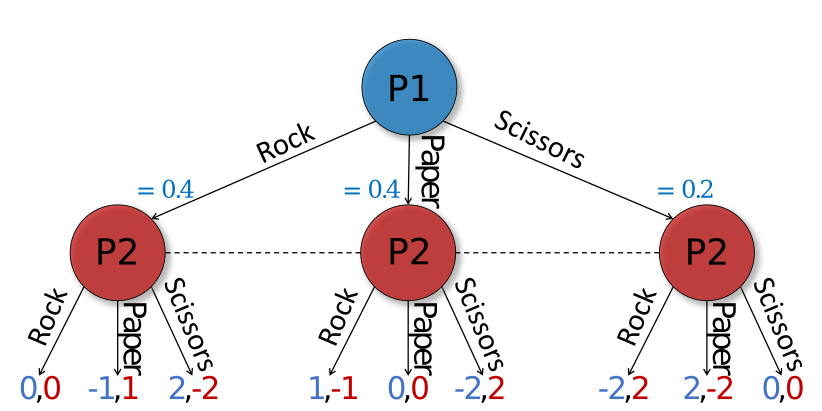
\includegraphics[width=0.6\textwidth]{./img/rsp.png}
  \caption{Drzewo decyzyjne dla algorytmu
  CFR \cite{iig}.}
\end{figure}

\subsection{Monte Carlo Conterfactual Regret Minimization}

W praktyce algorytm CFR przelicza całego drzewa decyzyjnego w jednej iteracji co tworzy wymagania
dużej mocy obliczeniowej. Dla małych gier takie rozwiązanie jest akceptowalne ale w przypadku 
wiekszych środowisk jest nie efektywny.
Spowodwało to powstanie nowszej wersji algorytmu - 'Monte Carlo Conterfactual Regret Minimization'
, który na każdą iterację eksploruje tylko część drzewa.
Jest on dobrym algorytmem do rozwiązania gier o średniej 
wielkości jak "Heads Up Limit Texas Poker Hold'em". 

Algorytm dzieli drzewo na n bloków gdzie każdy z nich zaczyna się od poczatkowego stanu t i
końcowego Z. Przy każdej iteracji zostaje wybrany jeden z nich, a nastepnie przeliczony. 
Metodę można podzielić na dwie odmiany, Outcome-Sampling MCCFR oraz External-Sampling MCCFR.

W metodzie zaimplementowanej w pracy została wykorzystana druga metoda. Polega ona na 
eksplorowaniu drzewa kolejno dla wszystkich graczy tak, że tylko dla oponentów jest przydzielana
jedna akcja w danym stanie na bazie dystrybucji akcji jakie posiada jego strategia \cite{mccfr}.



\chapter{Deep CFR}


W 2017 roku powstał algorytm Deep CFR rozwijający podstawową wersję metody CFR o sieci neuronowe.
Taka modyfikacjia była wymagana aby utworzyć algorytm, który morze rozwiązać nie tylko proste gry,
ale też i duże jak 'Heads Up Limit Poker Holdem'. Wylicza on wszystkie wartości w drzewie dezyzyjnym
przez algorytm MCCFR External-Sampling. Dodatkowo Deep CFR zbiega się do Równości Nasha szybciej niż 
popularny algorytm NFSP z 2016 roku \cite{dcfr}.


 

\begin{thebibliography}{100}
   \bibitem{Go} Gibney, Elizabeth. "Google AI algorithm masters ancient game of Go." Nature News 529.7587 (2016): 445.
   \bibitem{Dota2} Berner, Christopher, et al. "Dota 2 with large scale deep reinforcement learning." arXiv preprint arXiv:1912.06680 (2019).

   \bibitem{iig} Brown, Noam, et al. "Combining deep reinforcement learning and search for imperfect-information games." arXiv preprint arXiv:2007.13544 (2020).
   \bibitem{FSEG} Heinrich, Johannes, Marc Lanctot, and David Silver. "Fictitious self-play in extensive-form games." International conference on machine learning. PMLR, 2015.
   \bibitem{eq} Lockhart, Edward, et al. "Computing approximate equilibria in sequential adversarial games by exploitability descent." arXiv preprint arXiv:1903.05614 (2019).
   \bibitem{sp} Teófilo, Luís Filipe Guimarães. "Building a poker playing agent based on game logs using supervised learning." (2010).
   \bibitem {gm} Bouju, Gaëlle, et al. "Texas hold'em poker: a qualitative analysis of gamblers' perceptions." Journal of Gambling Issues 28 (2013): 1-28.
   \bibitem{class} Félix, Dinis Alexandre Marialva. "Artificial intelligence techniques in games with incomplete information: opponent modelling in Texas Hold'em." (2008).

   \bibitem{gt} Myerson, Roger B. Game theory. Harvard university press, 2013.
   \bibitem{rmg} Zinkevich, Martin, et al. "Regret minimization in games with incomplete information." Advances in neural information processing systems 20 (2007): 1729-1736.
   \bibitem{dcfr} Brown, Noam, et al. "Deep counterfactual regret minimization." International conference on machine learning. PMLR, 2019. 
   \bibitem{ds} Moravčík, Matej, et al. "Deepstack: Expert-level artificial intelligence in heads-up no-limit poker." Science 356.6337 (2017): 508-513. 
   \bibitem{ss} Davis, Trevor, Neil Burch, and Michael Bowling. "Using response functions to measure strategy strength." Twenty-Eighth AAAI Conference on Artificial Intelligence. 2014. 
   \bibitem{n} Heinrich, Johannes, Marc Lanctot, and David Silver. "Fictitious self-play in extensive-form games." International conference on machine learning. PMLR, 2015. 
   \bibitem{mccfr} Lanctot, Marc, et al. "Monte Carlo sampling for regret minimization in extensive games." Advances in neural information processing systems 22 (2009): 1078-1086.
\end{thebibliography}



\end{document}

